\section{Prototypes}

Tous le code présenté dans ce rapport est accessible ici: \url{https://github.com/Louis-Amas/Projet\_TER}

\begin{itemize}
    \item Phase de recherche.
    \item Comparaison avec une bibliothèque populaire.
    \item Comparaison avec le standard.
\end{itemize}

\subsection{Phase de recherche}

Pendant la phase de préparation du projet, je me suis renseigné sur toutes les manières de rendre un smart contract modifiable \emph{a posteriori}.
Mon temps de projet étant assez court, je me suis concentré sur une méthode nommée \emph{Proxy} \cite{PROXY}. Cette méthode permet de créer un
smart contract en façade qui déléguera les appels à un autre smart contract dit d'implémentation. J'ai aussi contacté
l'équipe de développement d'Ethereum afin d'obtenir plus de ressources. L'équipe de développement m'a répondu avec un document
contenant un récapitulatif de l'état de l'art sur la modification des smarts contracts. Une aubaine pour moi.

Ce document contenait de nombreux lien vers des répertoires Git, après quelques heures à lire le code source de ces répertoires,
et avec mes recherches en amont j'avais toutes les clefs nécessaires pour commencer. 

\subsection{Les outils}

Il me fallait un environnement de développement afin de commencer à programmer un prototype. L'Ethereum étant une technologie
décentralisée contenant plusieurs nœuds il est nécessaire d'utiliser des outils de simulation ou des réseaux de tests (Testnet).
J'ai opté pour la simulation de la blockchain Ethereum. J'ai utilisé la suite d'outil Truffle \cite{Truffle}.
%
Truffle contient un logiciel permettant d'émuler une blockchain Ethereum mais aussi, des bibliothèques pour gérer tout le cycle 
de vie des smarts contracts, développement, compilation, déploiement et test.

Truffle se présente sous la forme d'une interface de commande et d'une architecture de fichier spécifique. Truffle m'a été très
utile pour tester mes smarts contracts. En effet, il est possible d'écrire des tests automatiques en Javascript afin
de vérifier le bon fonctionnement des smarts contract.

Truffle peut aussi être connecté à une vraie blockchain et donc être utilisé en production. De plus, quelqu'un voulant comprendre
ou réutiliser mon code, pourra exécuter mon code une fois qu'il aura configuré la blockchain sur laquelle il souhaitera le déployér. Cela permet 
de simplifier l'environnement de développement. Durant ma phase
de recherche j'ai lu les tests Truffle des implémentations trouvés sur internet afin de mieux comprendre leurs fonctionnements.

L'outil Ganache \cite{Ganache} est aussi très utile pour débuger les smarts contracts car, il est possible de lire chaque transaction et chaque bloc de la blockchain simulé.

\subsection{Premier prototype}

Une fois tout en place j'ai pu commencer mon développement. J'ai décidé de commencer par l'implémentation d'un système de vote 
électronique comme décrit dans le scénario 1. J'ai programmé un système de vote simple permettant au créateur du vote de donner
le droit de voter a qu'il souhaite. Chaque utilisateur ayant le droit de vote peut alors voter pour un des candidats proposer par
le créateur du contrat. Je veux pouvoir avoir la possibilité de donner mon vote à quelqu'un d'autre, c'est-à-dire faire une 
procuration. Je souhaiterais pouvoir ajouter ou enlever dynamiquement cette fonctionnalité.

\subsubsection{Méthode utilisée}

Mon premier prototype réalise donc cette fonctionnalité. Pour réaliser cette modification alors que je rappelle 
qu'elle est normalement impossible car, les contrats sont immuable. J'ai utilisé une méthode appelée \texttt{Proxy}. Pour cela, j'ai créé un contrat avec quelque particularité. J'ai utilisé la fonction "\texttt{fallback()}" de Solidity. Cette fonction est appelée quand la fonction appelée sur un contrat n'existe pas. Cette fonctionnalité m'est très utile, car je vais pouvoir à l'aide de l'opcode \texttt{delegatecall} transmettre touts les appels fait au contrat \texttt{Proxy} au contrat contenant l'implémentation.

\begin{figure}[t!]
  \caption{Exemple de la méthode \texttt{Proxy}}
  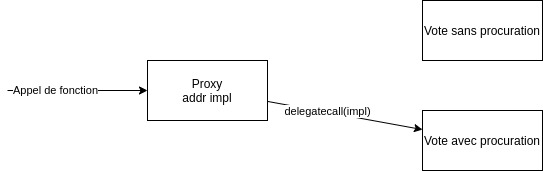
\includegraphics[scale=0.6]{proxy.jpg}
  \centering 
  \label{fig:proxy}
\end{figure}


\begin{figure}[!b!]
  \caption{Exemple de la méthode \texttt{Proxy} avec stockage structuré}
  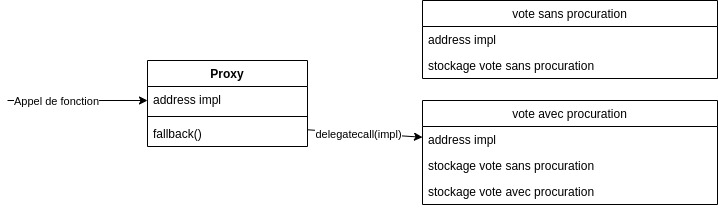
\includegraphics[scale=0.5]{proxy_structured_stockage.jpg}
  \centering 
  \label{fig:proxy_structure}
\end{figure}



\subsubsection{Détail technique}
L'opcode \texttt{delegatecall} permet d'exécuter du code se situant dans un autre contrat voir Figure \ref{fig:proxy}.  Il prend en paramètre une adresse d'un autre contrat.

Néanmoins, il est important de bien comprendre comment Solidity stocke les variables dans un contract, afin de 
comprendre comment  exécuter le code dans le contrat appelé par "\texttt{delegatecall}", peut-il interagir avec les variables.

En effet, l'opcode "\texttt{delegatecall}" à un comportement peu intuitif, \texttt{delegatecall} exécute le code d'un autre contrat mais garde le stockage du contrat appelant "\texttt{delegatecall}". Cela veut dire que le contrat implémentation doit savoir comment les variables du contrat appelant sont stockées.
%
Solidity stocke les variables les une après les autres 
%
$$\forall n \in N, var_1 \mapsto pos_1, var_2 \mapsto pos_2,
..., var_n \mapsto pos_n$$

Pour la réalisation d'un contrat \texttt{Proxy} il est nécessaire d'avoir une variable contenant l'adresse d'une implémentation, il est très important que le contrat contenant l'implémentation n'override pas son adresse.

Il existent deux méthodes pour s'assurer que cela n'arrive pas. La méthode la plus simple appelé  \emph{stockage structuré}, Figure \ref{fig:proxy_structure} et de mettre la variable contenant l'implémentation dans chaque contrat. 

La deuxième méthode appelé \emph{stockage non structuré}, Figure \ref{fig:proxy_unstructured}, est de stocker l'adresse de l'implémentation à une position "aléatoire".
Pour cela, on peut placer la variable à la position retournée par le calcul de la fonction sha3 sur le nom de la variable.
La fonction sha3 étant une fonction de hash il y a très peu de risque de collision.

La méthode avec un stockage non structuré est une meilleure solution car, elle permet d'utiliser des contrats d'implémentation qui ne connaisse pas l'existence du \texttt{Proxy}.

\begin{figure}[!t!]
  \caption{Exemple de la méthode \texttt{Proxy} avec stockage non structuré}
  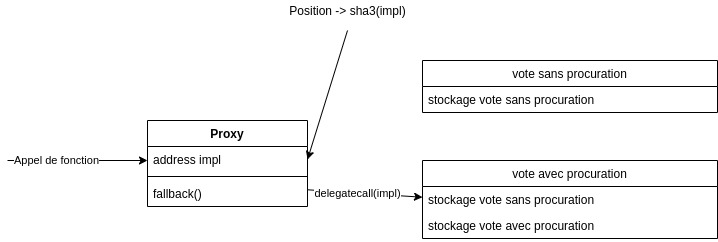
\includegraphics[scale=0.4]{proxy_unstructured.jpg}
  \centering 
  \label{fig:proxy_unstructured}
\end{figure}

\subsection{Implémentation officielle (Diamond)}

En poursuivant mes recherches sur l'état de l'art du domaine j'ai trouvé sur le site internet des 
"Ethereum Improvement Proposals"(EIP) \cite{EIP}. La proposition 2535 du 22 février 2020 ayant pour but de formaliser
la manière dont programmer un \texttt{Proxy} ``intelligent''. Le principe sous-jacent est identique à mon prototype
avec un stockage non structuré mais, cette proposition y ajoute une interface plus simple et plus modulable.

En effet, l'objectif est de créer une bibliothèque avec une interface simple afin de permettre facilement à un
utilisateur de programmer son propre proxy personnalisé a forme de ``\emph{diamant}'': ce diamant fonctionne de la manière suivante.

Un diamant est composé de facette chaque facette représente une fonction. Chaque facette permet de lier l'identificateur
de fonction à l'adresse d'un autre contrat. Quand un appel de fonction est exécuté sur un diamant alors celui-ci ira chercher
dans sa structure de données la facette correspondante à l'appel de fonction. Une fois cette facette trouvée il pourra alors
appeler \texttt{delegatecall} sur l'adresse associé à cette facette afin d'exécuter le coder situé dans un autre contract.

Afin d'ajouter, modifier ou supprimer une facette la bibliothèque proposée contient une fonction nommée "diamondCut". Cette fonction prend en paramètre un tableau de "coupe de diamant". Une coupe de diamant est une structure contenant
une action (Ajouter, modifier ou supprimer), une adresse d'un contract et un tableau de sélecteur de fonction. Voir la Figure
\ref{fig:diamond_struct}

Un développeur voulant utiliser cette bibliothèque aura juste à générer un tableau de "coupe de diamant" modélisant le 
proxy qu'il souhaite réaliser. La seule obligation du développeur est d'utiliser uniquement un stockage non structuré dans
ces facettes.

\begin{figure}[h]
  \caption{Schéma représentatif du fonctionnement internet d'un diamant.}
  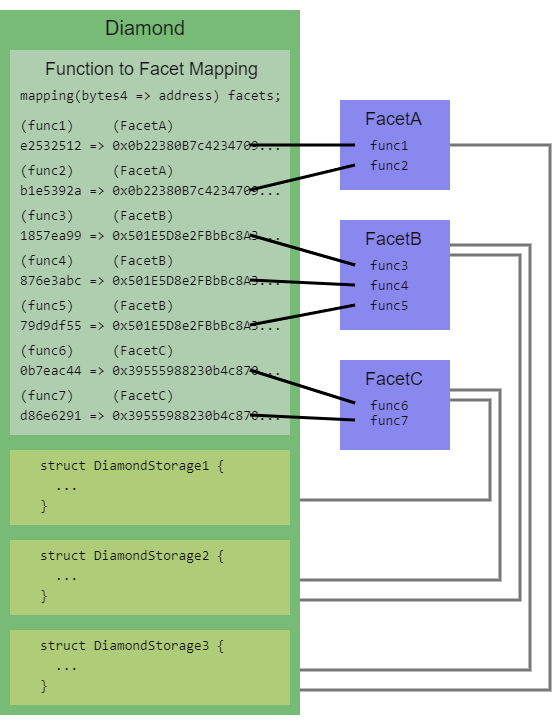
\includegraphics[scale=0.5]{diamond_struct.png}
  \centering 
  \label{fig:diamond_struct}
\end{figure}

\begin{figure}[h]
  \caption{Schéma représentatif des appels à un diamant.}
  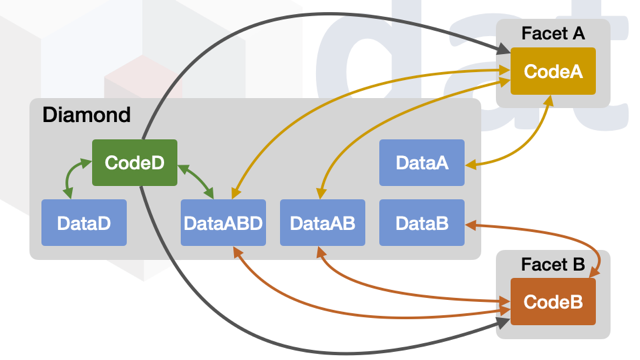
\includegraphics[scale=0.5]{diamond_ex.png}
  \centering
  \label{fig:diamond_ex}
\end{figure}


\subsection{Comparaison de mon prototype et du diamant}

Il est évident que l'implémentation officielle est bien plus avancée que mon prototype,
néanmoins nous pouvons voir que mon prototype utilise la même technique que l'implémentation officielle.
La plus grande différence entre le diamant et mon prototype est la modularité. En effet, mon prototype étant
un prototype je ne me suis pas concentré sur la simplicité de l'interface d'utilisation. Mon objectif était 
de réaliser un "Proof of Concept". L'objectif est réalisé, j'ai un prototype fonctionnel et cela m'a permis 
de bien mieux comprendre le fonctionnement de l'implémentation officielle. J'ai pu acquérir les connaissances
bas niveaux nécessaires à de telle utilisation.
